\chapter{OpenStack Architecture}
\label{ch:arch}
This chapter describes the OpenStack architecture, how the components communicate and what they are used for. Selected components, which are needed for the deployment option used later in this thesis, will be described in more detail.

\section{Conceptual Architecture}
Conceptual architecture is a high level architecture that shows the core components of a system and their relations including description of responsibilities for each component.

The relationships among the OpenStack services can be seen on picture \ref{fig:OpenStack_conceptual_arch}.
\begin{figure}[!h]
  \includegraphics[width=\textwidth]{fig/OpenStack_conceptual_arch.png}
  \caption{OpenStack conceptual architecture [Source: \cite{conceptualArch}]}
  \label{fig:OpenStack_conceptual_arch}
\end{figure}





\section{Logical Architecture}
Logical architecture shows processes and functions that make the system functioning.

OpenStack consists of several independent parts called OpenStack services.\cite{CL210} Authentication for all services is provided by a common identity service. The services interact with each other via public APIs. \cite{AdminGuide}

OpenStack services are internally composed of several processes. Each service has at least one API process. This API process listens for API requests, does necessary preprocessing and passes them to the particular process or processes within the service. The actual work of a service is done by distinct processes. An exception to this rule is the identity service.

The processes within a service communicate with each other via message broker using AMQP protocol. The most used AMQP broker is RabbitMQ, which is also used in this thesis.

The state of a service is stored in a database. OpenStack support several databases, such as MySQL, MariaDB, and SQLite. The database solution used in this thesis is MariaDB. \cite{AdminGuide}

Users can interact with OpenStack in several ways. There is a graphical web-based interface, which is implemented by OpenStack Dashboard. Other ways include command-line clients provided by all basic services, and by API requests using web browser plugins or curl.

The most common, but not the only possible logical architecture can be seen on picture \ref{fig:OpenStack_logical_arch}.

\begin{figure}[!h]
  \centerline{\includegraphics[width=14cm]{fig/OpenStack_logical_architecture_2.png}}
  \caption{OpenStack logical architecture [Source: \cite{OperationsGuide}]}
  \label{fig:OpenStack_logical_arch}
\end{figure}

\section{Physical Architecture}
OpenStack is a distributed system, which enables cloud architects to design varieties of physical architecture reflecting needs of the cloud consumer.

\textit{“Designing an OpenStack cloud is a great achievement. It requires a robust understanding of the requirements and needs of the cloud’s users to determine the best possible configuration to meet them. OpenStack provides a great deal of flexibility to achieve your needs...”} \cite{OperationsGuide}




\section{Installation of Core Components}

This section will explain each service of the OpenStack cloud in more detail including general description, some basic principles of the function, and a list of components of the service. Some services, such as Compute or Storage, can use several backends for the actual work. List and short description of these backends is also included in this section.


\subsection{OpenStack Identity Service}
The OpenStack identity service provides a single point of authentication and authorisation. When OpenStack services receive a request from a user, they check with the identity service to verify the authorisation of the user.

It also provides a catalog of OpenStack services. When installing OpenStack cloud, each service needs to be registered in the identity service. The identity service then tracks which services are installed and where they are located on the network.

OpenStack services also use the identity service as a common unified API.

\subsubsection*{Identity Abstractions}

The identity service uses the following abstractions:
\begin{itemize}
  \item{\textbf{Service} is an OpenStack service, such as the identity (Keystone) service, compute (Nova) service, etc.}
  \item{\textbf{Endpoint} is an address accessible via network and acts as an access-point of a service.}
  \item{\textbf{Region} represents a general division of the OpenStack deployment. The identity service also supports sub-regions, which allows the creation of a tree-structured hierarchy.}
  \item{\textbf{Authentication} is the process of confirming the identity of a user. To confirm an incoming authentication request, the identity service validates a set of credentials supplied by the user. These can be a name and password, or a name and API key. After validation of the user credentials, the identity services then issues an authentication token. This process is done only once on in the beginning of a session and user then provide this token in all subsequent requests.}
  \item{\textbf{Credentials} are data to identify the user, such as name and password, or name and API key.}
  \item{Authentication \textbf{token} is an alpha-numeric string used to access to OpenStack APIs and resources. Token is valid for a finite duration and can be revoked at any time.}
  \item{\textbf{Domain} is a collection of projects and users. This collection defines administrative boundaries for managing identity entities. Domains can be used to represent an individual person, a company, or an operator-owned space. User can be granted the administrator role within a domain. This domain administrator can then create users, projects, and groups in the domains as well as create and assign roles to users or groups.}
  \item{\textbf{Project} is used to isolate resources or identity objects. Projects can be used to map to a customer, account, organisation, or tenant.}
  \item{\textbf{Role} is a personality containing a set of user rights and privileges. A user contains a list of roles.}
  \item{\textbf{Group} is a collection of users and is owned by a domain. A group can be assigned a role that applies to all users in the group.}
  \item{\textbf{User} is a representation of a person, system or service using the OpenStack services.}
  \\\cite{CL210}
\end{itemize}


\subsubsection*{OpenStack Identity Components}

The identity service consists of these components:
\begin{itemize}
  \item{\textbf{Server} - A centralised server, providing authentication and authorisation services. It uses a RESTful interface.}
  \item{\textbf{Drivers} - Drivers are used to access identity information provided by external repositories like LDAP, or existing SQL databases.}
  \item{\textbf{Modules} - Middleware modules that check service requests, extract user credentials and send them to the Server for authorisation. The modules are integrated with the OpenStack components by using the Python Web Server Gateway Interface (Python WSGI).}
 \\\cite{InstallGuide}
\end{itemize}


\subsection{OpenStack Image Service}
The OpenStack Image service controls image storage and management and allows users to discover, register, and retrieve images.

Images provide templates for virtual machine filesystems. Each virtual machine runs from a copy of a base image and several virtual machines can be run from a single base image. Any changes made to the virtual machines will not affect the image. Users can also create a snapshot - a state of a virtual machines running disk - and build a new image based on these snapshots.

The implementation of the image service is called Glance. It supports various backends as a storage, which can be normal filesystems, OpenStack object storage, HTTP, RADOS block devices, and Amazon S3. Some of the storage backends can be read-only. The architecture in this thesis will use normal filesystem mounted to the controller node.

\subsubsection*{Basic Components}
The image service consists of the following components:
\begin{itemize}
  \item{\textbf{glance-api} - Accepts API calls.}
  \item{\textbf{glance-registry} - Stores, processes, and retrieves metadata about images like size and type. This is an internal service only and should not be exposed outside of the image service.}
  \item{\textbf{Database} - An SQL database to store image metadata.}
  \item{\textbf{Storage} repository for image files - Backend that stores the images itself.}
\end{itemize}





\subsection{OpenStack Compute Service}
The OpenStack Compute service is the major part of an Infrastructure as a Service (IaaS) system. It runs and manages the virtual machines running in the OpenStack cloud. It can also provide networking for the virtual machines. However, Nova networking is not often used. The OpenStack Networking (Neutron) , described in this section, is used instead. \cite{InstallGuide}

The OpenStack Compute service scales horizontally and is commonly deployed on multiple hosts, \cite{OperationsGuide} often called compute nodes.

The service manages virtualisation, but it does not include any virtualisation software. Instead, it uses drivers to interact with the underlying virtualisation backend, also called virtualisation provider. It is also possible to use multiple providers in different availability zones.

The OpenStack Compute service supports these following virtualisation providers: \cite{AdminGuide}
\begin{itemize}
  \item{Baremetal}
  \item{Docker}
  \item{Hyper-V}
  \item{Kernel-based Virtual Machine (KVM)}
  \item{Linux Containers (LXC)}
  \item{Quick Emulator (QEMU)}
  \item{User Mode Linux (UML)}
  \item{VMware vSphere}
  \item{Xen}
\end{itemize}

\subsubsection*{Service Architecture}

The architecture of the Compute service could be divided into the following four parts:
\begin{itemize}
  \item{\textbf{API Server} is the compute controller that commands and controls the hypervisor, storage, and networking available to the end users. It manages the API endpoints, which are basic HTTP web services that handle the authentication, authorisation, and basic command and control functions. It support various API interfaces including Amazon, Rackspace, and others, which enables compatibility with multiple existing tools already created for other cloud platforms. This open approach also prevents vendor lock-in.}
  \item{\textbf{Message Queue} manages the interaction between compute nodes, the networking controllers, API server, and the scheduler. It is provided by the Advanced Message Queuing Protocol (AMQP). Several implementations are available, the most common are RabbitMQ, Qpid, ZeroMQ, and others.}
  \item{\textbf{Compute Worker} manages the virtual machines that run on the compute nodes. It is managed via API that provides commands to run, delete, and reboot instances, attaching and detaching volumes, and to get local console output.}
  \item{\textbf{Network Controller} manages the networking resources available on the compute nodes. It is managed via API that provides commands for allocating fixed IP addresses, configuring VLANs for projects, or configuring networks for compute nodes.}
  \\\cite{AdminGuide}
\end{itemize}

\subsubsection*{OpenStack Compute Components}

The OpenStack Compute service consists of the following components:
\begin{itemize}
  \item{\textbf{\texttt{nova-api} service} - Accepts API calls and responds to them. It supports the OpenStack Compute API, the Amazon EC2 API, and a special Admin API.}
  \item{\textbf{\texttt{nova-api}-metadata service} - Accepts metadata requests from instances.}
  \item{\textbf{\texttt{nova-compute} service} - A worker daemon that manages virtual machines via virtualisation provider API. It supports XenAPI, libvirt, VMwareAPI, and others. The state of the instances is always saved in the database.}
  \item{\textbf{\texttt{nova-scheduler} service} - This service determines on which compute node a new virtual machine should be started.}
  \item{\textbf{\texttt{nova-conductor} module} - It is a point of access to the database for other nova services. It eliminates direct access to the database by other services. This service scales horizontally and can be deployed on multiple hosts.}
  \item{\textbf{\texttt{nova-cert} module} - This is only needed to use with the Amazon EC2 API, used to generate certificates.}
  \item{\textbf{\texttt{nova-network} worker daemon} - Similar to the nova-compute service, but for networking. Accepts networking tasks from the queue and manipulates the network.}
  \item{\textbf{\texttt{nova-consoleauth} daemon} - Provides authorisation for users provided by the console proxies - see nova-novncproxy and nova-xvpvncproxy for more information. It needs to run for the proxies to work.}
  \item{\textbf{\texttt{nova-novncproxy} daemon} - Proxy for accessing running virtual machines via a VNC connection. Supports browser-based HTML5 clients.}
  \item{\textbf{\texttt{nova-spicehtml5proxy} daemon} - Proxy for accessing running virtual machines via a SPICE connection. Supports browser-based HTML5 clients.}
  \item{\textbf{\texttt{nova-xvpvncproxy} daemon} - Proxy for accessing running virtual machines via a VNC connection. Supports an OpenStack-specific Java client.}
  \item{\textbf{\texttt{nova-cert} daemon} - Manages x509 certificates.}
  \item{\textbf{\texttt{euca2ools} client} - A set of command-line interpreter commands to manage the cloud resources via Amazon EC2 interface.}
  \item{\textbf{\texttt{nova} client} - A command-line client for the end user.}
  \item{\textbf{Message Queue} - Passes messages between nova daemons. Provided by the Advanced Message Queuing Protocol (AMQP). It is usually implemented by RabbitMQ.}
  \item{\textbf{SQL Database} - Stores most of the build-time and run-time states of the infrastructure, including information about available virtual machine types, virtual machines in use, available networks, and information about projects. OpenStack Compute supports SQLite3 for test and development work, MySQL and MariaDB, and PostgreSQL.}
  \\\cite{InstallGuide}
\end{itemize}



\subsection{OpenStack Networking Service}
The OpenStack Networking service enables users to create virtual networks and attach the devices managed by other OpenStack services to them. It provides an API that lets users to configure and manage network connectivity and addressing. The network services include L3 forwarding, NAT, load balancing, firewalls, and VPN.

Networking provides the end users the ability to create virtual networks, subnets, routers, and firewalls. All of these will be explained later in this section.

It also supports variety of plug-ins which can enable interoperability with several commercial and open source technologies. This plug-in architecture provides flexibility when designing custom OpenStack architecture and deploying it.

\subsubsection*{Networking}
Before using or deploying the OpenStack Networking service, the following general facts about networking \cite{NetworkingGuide} should be understood:

\begin{itemize}
  \item{\textbf{Ethernet} is a networking protocol that is being used by most wired network interface cards. In the OSI model of networking, Ethernet operates on the second layer, also referred to as layer 2, L2, link layer, or data link layer. Every host has unique identification called Media Access Control (MAC) address.

  Ethernet can be conceptually think of as a single bus, to which each of the network host is connected. However, modern networks use devices called switches, and every device is connected directly to them.

  The OpenStack Dashboard uses this simple model to visualise the network topology to the end user. This ethernet network is sometimes referred to as a layer 2 segment.}
  \item{\textbf{VLAN} is a networking technology that creates separate virtual network on a single switch in a way, that devices connected to the same switch can not each other's traffic, if they are on different VLANs.

  OpenStack uses VLANs to isolate the traffic of different tenants, even when their instances run on a single host.

  Each VLAN has a numerical ID between 1 and 4095. For example, a VLAN with an id of 15 will be referred to as VLAN 15.}
  \item{\textbf{Address Resolution Protocol (ARP)} - As pointed out above, network devices use MAC addresses to be identified. However, TCP/IP applications use IP addresses as an identifiers. The Address Resolution Protocol (ARP) bridges the gap by translating IP addresses into MAC addresses.}
  \item{\textbf{Dynamic Host Configuration Protocol (DHCP)} dynamically assigns IP addresses to network hosts. These hosts are called DHCP clients.}
  \item{\textbf{TCP, UDP, and ICMP} - Software applications communicating over an IP network use another protocols above IP. In the OSI model of networking, they use the fourth layer, which is also referred to as layer 4, or transport layer. There are three main protocols:
    \begin{itemize}
      \item{\textit{Transmission Control Protocol (TCP)} is the most commonly used layer 4 protocol. It is a connection-oriented protocol. Delivery of packets via this protocol is guaranteed.}
      \item{\textit{User Datagram Protocol (UDP)} is mostly used to transfer real-time information like voice or video. It is a connectionless and unreliable protocol which means that the delivery of packaets via this protocol is not guaranteed.}
      \item{\textit{Control Message Protocol (ICMP)} is used for sending control messages.}
    \end{itemize}
  }
  \item{\textbf{Switch} is device that allow packets to travel from one node to another. They connect hosts belonging to the same layer-2 network. Switches forward the traffic based on the destination Ethernet address in the packet header.}
  \item{\textbf{Router} is device that allows communication between nodes on different layer-3 networks. They route the traffic based on the destination IP address in the packet header.}
  \item{\textbf{Firewall} is device that restricts traffic to and from hosts on a network by special rules defined on the device. They are supposed to protect hosts from unauthorised access and attacks.}
  \item{\textbf{Load Balancer} is device that allows even distribution of traffic across several hosts. They are supposed to avoid overload of a single host. They also prevent a single point of failure as they enable the traffic to be processed by multiple hosts.}

\subsubsection*{Networking Concepts in OpenStack}
OpenStack uses the following concepts to enable users to create their own virtual network infrastructure:
  \item{\textbf{Network} is an isolated L2 segment. There are two types of network:
    \begin{itemize}

      \item{\textit{Tenant Networks} are managed by the end user and are used within their projects. These networks are fully isolated from other projects.}
      \item{\textit{Provider Networks} are managed by the OpenStack administrator and map ti the existing physical network in the datacenter. These networks are mainly used to enable external connectivity to the virtual machines running in the cloud. Each project should have at least one public provider network.}
    \end{itemize}
    }
  \item{\textbf{Subnet} is a block of IP addresses and associated configuration state. They are used to allocate IP addresses to ports that are created on a network.}
  \item{\textbf{Port} - Not to be confused with TCP or UDP port. In the OpenStack terminology, port is a connection point for attaching a single device (such as NIC of a virtual machine) to a virtual network. It also describes the configuration like MAC address and IP address.}
  \item{\textbf{Security Groups} enable users to define their own firewall rules in groups. They can control traffic in both direction (called ingress and egress). These rules are then applied to a port. A port can be assigned with multiple security groups.}
  \\\cite{NetworkingGuide}
\end{itemize}

\subsubsection*{OpenStack Networking Components}
The OpenStack Networking service is composed of the following components \cite{InstallGuide}:
\begin{itemize}
  \item{\textbf{neutron-server} - accepts API requests and routes them to the appropriate Networking plug-in}
  \item{\textbf{OpenStack Networking plug-ins and agents} - the main logic is implemented by several plug-ins. They plug and unplug ports, create networks, subnets, and provide IP addressing. OpenStack Networking ships with plug-ins and agents for Cisco virtual and physical switches, NEC OpenFlow products, Open vSwitch, Linux bridging, and the VMware NSX product. The architecture in this thesis will use Linux bridging.}
  \item{\textbf{Messaging queue} - routes the information between neutron-server and other agents. It also act as a database for particular plug-ins. The architecture in this thesis will use centralised RabbitMQ service running on a controller node.}
\end{itemize}

The architecture in this thesis will use the following plug-ins and agents for networking:
\begin{itemize}
  \item{\textbf{Modular Layer 2 plug-in} - builds layer-2 (bridging and switching) virtual networking infrastructure for virtual machines. IT uses the Linux bridge mechanism.}
  \item{\textbf{Linux bridge agent} - builds the networking infrastructure for virtual machines and also manages VXLAN tunnels for private networks and security groups.}
  \item{\textbf{Layer 3 agent} - is the most commonly used agent that provides layer-3 (routing) services for virtual networks.}
  \item{\textbf{DHCP agent} - provides DHCP services for virtual networks.}
\end{itemize}







\subsection{OpenStack Block Storage Service}
The OpenStack Block Storage service adds persistent block storage to a virtual machine instances and provides an infrastructure for managing volumes. This service is similar to the Amazon EC2 Elastic Block Storage (EBS) offering.

The service supports various backends which can be consumed using a Block Storage driver. An example of supported drivers that are available can be NAS/SAN, NFS, iSCSI, Ceph, and more. A usage of multi-backend configuration is also supported. \cite{InstallGuide}

To install the OpenStack Block storage service, it is important to understand a number of concepts, because there are several choices of deployment. \cite{OperationsGuide} Apart from choosing the right storage backend, it mostly depends on the final architecture - which can be single node or multi-node. For example, in this thesis I use a multi-node architecture with separate block storage node, and will use a local LVM storage as a backend.

\subsubsection*{Logical Volume Management (LVM)}
Because this thesis will use an LVM as a block storage provider, it is important to understand the basic concepts of LVM.

LVM creates a layer of abstraction over physical storage, which allows you to create multiple logical storage volumes. From an application view, these logical volumes are the same as traditional disk partitions. The hardware storage configuration is also hidden from the software, so it can be resized and moved without stopping services or unmounting filesystems. And in an opposite way, the logical volumes can be also resized without changing the underlying physical storage. This solution provides much more flexibility than using traditional partitions directly. \cite{LVMPdf}

\begin{figure}[!h]
  \centerline{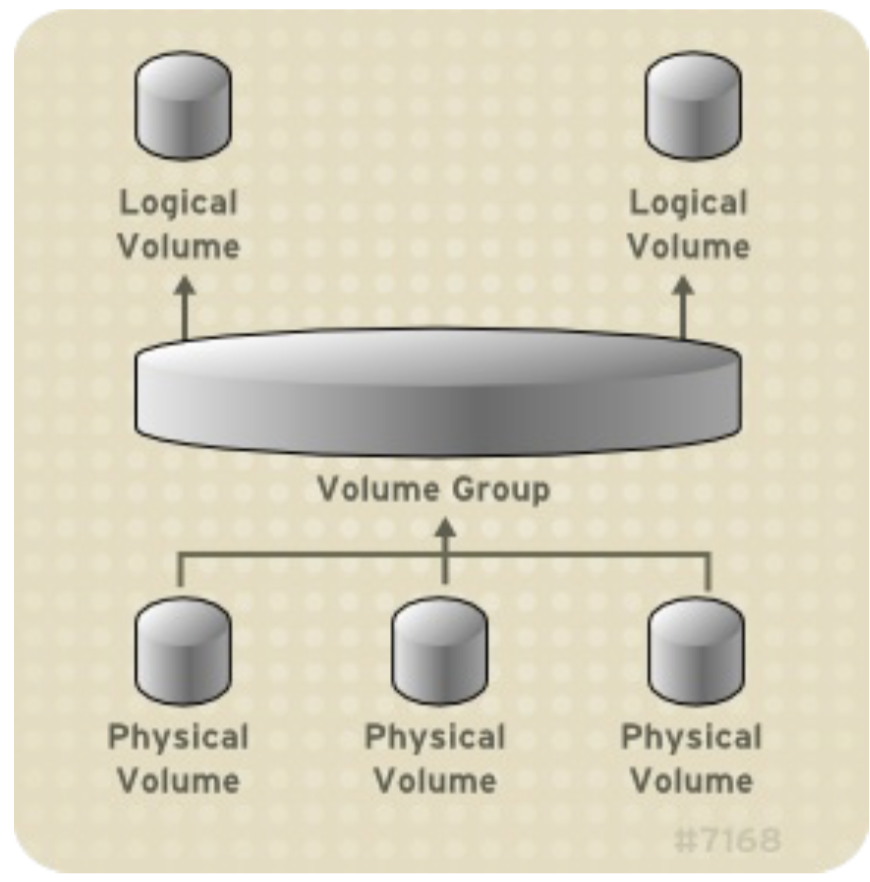
\includegraphics[width=8cm]{fig/lvm_architecture.png}}
  \caption{Logical volume architecture [Source: \cite{LVMPdf}]}
  \label{fig:lvm_architecture}
\end{figure}

As shown on the picture \ref{fig:lvm_architecture}, LVM consists of three basic layers:
\begin{itemize}
\item{\textbf{Physical Volume (PV)} is the underlying physical block storage device, which can be a partition or the whole disk. To use the device for LVM, it needs to be initialised as a Physical Volume (PV).}
\item{\textbf{Volume Group (VG)} is a combination of several physical volumes. However, volume group can also consist of a single physical volume. This layer provides a pool of disk space used to create logical volumes (LV) in the same way disks are divided into partitions.}
\item{\textbf{Logical Volume (LV)} is the volume used by filesystems and applications. In LVM, a volume group is divided into several logical volumes.}
\end{itemize}

\subsubsection*{Block Storage Components}

The OpenStack Block Storage service consists of the following components \cite{InstallGuide}:
\begin{itemize}
\item{\textbf{cinder-api} - Accepts API requests and routes them to the cinder-volume process for action.}
\item{\textbf{cinder-volume} - This process manages the read and write requests sent to the Block Storage service. It interacts with the cinder-scheduler and cinder-backup processes and the storage providers, using respective drivers.}
\item{\textbf{cinder-scheduler daemon} - In multi-node deployments, it selects the optimal storage node on which the volume will be created. This process is similar to the nova-scheduler.}
\item{\textbf{cinder-backup daemon} - Provides the ability to back up volumes. It can interact with multiple backup storage providers using drivers, in a similar way as the cinder-volume process.}
\item{\textbf{Messaging queue} - Routes information between the processes within the OpenStack Block Storage service. In this thesis, I use a centralised RabbitMQ service, running on the controller node.}
\end{itemize}




\subsection{OpenStack Dashboard Service}
The OpenStack Dashboard service provides you a way to manage the OpenStack resources and services. It is used by administrators and the end user. It provides a web-based interface that communicates through the OpenStack APIs. It also allows customising the brand of the dashboard to match the cloud provider's needs. \cite{InstallGuide}

\subsubsection*{Handling of User Session Data}

The Dashboard service supports several session backends \cite{DeployingHorizon} to handle the user session data:
\begin{itemize}
  \item{\textbf{Local Memory Cache} - The quickest and easiest session backend, which does not require external dependencies and is the easiest to set up. However, it does not support shared storage across processes or workers, and does not offer data persistency after a process terminates. This is the reason why it is not recommended for production use.}
  \item{\textbf{Memcached} - An external caching service. Supports shared storage and offers data persistency after process or worker terminates. It is extremely fast and efficient cache backend. It requires the memcached service to be running and accessible and a python memcached module installed.}
  \item{\textbf{Database} - A database can be also used as a caching backend. It is scalable, it can be highly-available and offers data persistency. However, it is slow in comparison to other caching methods.}
  \item{\textbf{Cached Database} - This is a hybrid setting using database and caching infrastructure together.}
  \item{\textbf{Cookies} - Stores data in a cookie in the user's browser. It supports a cryptographic signing to ensure that the data has not been changed during transport. It should be noted, that signing is not the same as encryption, so that the data are still readable by potential attacker.}
\end{itemize}

In this thesis, I will use the Memcached option.
